\documentclass[11pt, english, fleqn, DIV=15, headinclude, BCOR=2cm]{scrreprt}

\usepackage[
    color,
    bibatend,
]{../../header}

\graphicspath{{_build/}{../Figures/}}

\hypersetup{
    pdftitle=
}

\subject{Lab report}
\title{Mößbauer effect}
\subtitle{Experiment K221 -- Universität Bonn}
\author{%
    Martin Ueding \\
    \small{\href{mailto:mu@martin-ueding.de}{mu@martin-ueding.de}}
    \and
    Lino Lemmer \\
    \small{\href{mailto:l2@uni-bonn.de}{l2@uni-bonn.de}}
}

\date{2016-03-02}

\publishers{Tutor: Peter Klassen}

\begin{document}

\maketitle

\chapter*{Permission to upload}

I, Martin Ueding, would like to scan and upload this lab report with your
corrections to my website \href{http://martin-ueding.de}{martin-ueding.de}.
There, the original lab report as well as the reviewed one will be licensed
under the “\href{http://creativecommons.org/licenses/by-sa/4.0/}{Creative
Commons Attribution-ShareAlike 4.0 International License}”. Is that okay with
you?

Yes $\Box$ \hspace{2cm} No $\Box$

\begin{abstract}
\end{abstract}

\tableofcontents

\chapter{Theory}

\section{Absorption and resonances}

Like the electrons in an atom, the constituents of a nucleus also have
excited states and associated energy levels. As the nucleus is orders of
magnitude smaller than the whole atom, the relevant energies are orders of
magnitude larger. The hydrogen transition energies are in the order of
\SIrange{1}{10}{\electronvolt} whereas the transition energies cobalt and iron
are in the order of \SIrange{10}{100}{\kilo\electronvolt}.

If the energy matches an allowed transition, a nucleus can also absorb
electromagnetic radiation and transition into an excited state. As most nuclei
in a metal are in the groundstate, the highest absorption can be obtained by a
transition from the groundstate. Photons with the required energy are created
by an excited nucleus of the same isotope decaying into the groundstate.

The experimental setup here will have a radiation source made from cobalt. This
decays into excited iron via electron capture (EC), see Figure~\ref{fig:ec}.
The excited nucleus in turn will decay into the groundstate via some
metastable states. See Figure~\ref{fig:co57} for the decay scheme of the
radioactive material used in this experiment. The transition into the
groundstate is the one from $3/2^-$ to $1/2^-$ with an energy gap of $\hbar
\omega = \SI{14.4}{\kilo\electronvolt}$.

\begin{figure}
    \centering
    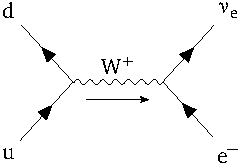
\includegraphics{ec}
    \caption{%
        Electron capture, leading order contribution.
    }
    \label{fig:ec}
\end{figure}

\begin{figure}
    \centering
    \includegraphics{co57}
    \caption{%
        Decay scheme of $^{57}\mathrm{Co}$ into $^{57}\mathrm{Fe}$. Cobalt from
        the source undergoes electron capture (EC) with a very long halftime.
        The transition between to the groundstate (thick) is the Mößbauer
        energy level we are interested in.
        %
        Figure adapted from
        \textcite[Abb.~4.8]{Schatz/Nukleare_Festkoerperphysik}.
    }
    \label{fig:co57}
\end{figure}

The emission lines are not perfectly sharp. This limits the chance of
absorption by the same kind of nucleus. The broadening effects are the
following:

\begin{description}
    \item[Natural width]
        The lifetime $\tau$ of every metastable state is limited. If it were
        not, one would not observe the transition. Together with the
        energy-time-uncertainty this directly leads to a line width of
        \[
            \Gamma = \frac\hbar\tau \,.
        \]
        Our line of interest, the \SI{14.4}{\kilo\electronvolt}-line has a
        lifetime of \SI{141}{\nano\second} and therefore a width of $\Gamma =
        \SI{4.7e-9}{\electronvolt}$. Compared to energy of the photons
        themselves, this is a relative width of \num{3.3e-13} which is very
        small compared to the other effects.
        \parencite[42]{Schatz/Nukleare_Festkoerperphysik}

    \item[Doppler effect]
        A relative motion between source and target will lead to a Doppler
        shift. The Lorentz transformation connecting the two systems boosts the
        photon's energy. If the source particles are subject to thermal
        motions, the spectrum will be broadened. At room temperature the shifts
        in energy are around \SI{10e-2}{\electronvolt}
        \parencite[43]{Schatz/Nukleare_Festkoerperphysik}, depending on the
        angle of motion and emission.

        The natural line width could be ignored when the Doppler effect is
        present.

    \item[Recoil]
        The photon carries momentum $\hbar k$. In the center of mass frame of
        the emitting nucleus, the nucleus will take the recoil $- \hbar k$. The
        energy of the nucleus then is
        \[
            \frac{[\hbar k]^2}{2 M} \,
        \]
        where $M$ is the mass of nucleus. This energy is subtracted from the
        photon; the photon has a reduced frequency when emitted from a free
        nucleus.
\end{description}

Taking all those effects together, it becomes unlikely that the photons emitted
by a gas of decaying cobalt will be absorbed by a gas of iron, ignoring that it
might be impractical to realize this situation. The issue of the recoil can be
reduced by embedding the nuclei of interest into a solid. The lattice will
absorb the excess momentum and due to its practically infinite mass (\num{e23}
larger), there will be no recoil velocity and therefore no energy shift in the
photon.

\section{Hyperfine structure}

The angular momentum $l$ and the spin $s$ of the nucleus couple to a combined
spin $j$. The component along the quantization axis, $m_j$, takes values
between $-j$ and $j$. The various states organize them into the irreducible
representations of $\SU(2)$, the multiplets with spin $j$ and $(2j+1)$ states
each. The different multiplets have different energies, the energies within the
same multiplet are degenerate, see left part of Figure~\ref{fig:M1}. Breaking
the $\SU(2)$ symmetry of the spins give the nuclear analogue of the Zeeman
effect. The degeneracy is broken and each multiplet is split up into
equidistant levels, see the right part of said figure.

\begin{figure}
    \centering
    \includegraphics{M1}
    \caption{%
        Hyperfine structure of the \SI{14.4}{\kilo\electronvolt}-M1-line in
        $^{57}\mathrm{Fe}$, our Mößbauer transition.
        Figure adapted from
        \textcite[Abb.~4.22]{Schatz/Nukleare_Festkoerperphysik}.
    }
    \label{fig:M1}
\end{figure}

\end{document}

% vim: spell spelllang=en tw=79
